\subsection{Full-Round Actions}

\Table{Full-Round Actions}{LZ{14mm}}{
\tableheader Action & \tableheader Attack of Opportunity\footnotemark[1] \\
Full attack & No \\
Charge\footnotemark[2] & No \\
Deliver coup de grace & Yes \\
Escape from a net & Yes \\
Extinguish flames & No \\
Light a torch & Yes \\
Load a heavy or repeating crossbow & Yes \\
Lock or unlock weapon in locked gauntlet & Yes \\
Prepare to throw splash weapon & Yes \\
Run & Yes \\
Use skill that takes 1 round & Usually \\
Use touch spell on up to six friends & Yes \\
Withdraw\footnotemark[2] & No \\
\TableNote{2}{1 Regardless of the action, if you move out of a threatened square, you usually provoke an attack of opportunity. This column indicates whether the action itself, not moving, provokes an attack of opportunity.}\\
\TableNote{2}{2 May be taken as a standard action if you are limited to taking only a single action in a round.}\\
}

A full-round action requires an entire round to complete. Thus, it can't be coupled with a standard or a move action, though if it does not involve moving any distance, you can take a 1.5-meter step.

\subsubsection{Full Attack}
If you get more than one attack per round because your base attack bonus is high enough, because you fight with two weapons or a double weapon or for some special reason you must use a full-round action to get your additional attacks. You do not need to specify the targets of your attacks ahead of time. You can see how the earlier attacks turn out before assigning the later ones.

The only movement you can take during a full attack is a 1.5-meter step. You may take the step before, after, or between your attacks.

If you get multiple attacks because your base attack bonus is high enough, you must make the attacks in order from highest bonus to lowest. If you are using two weapons, you can strike with either weapon first. If you are using a double weapon, you can strike with either part of the weapon first.

\textbf{Deciding between an Attack or a Full Attack:} After your first attack, you can decide to take a move action instead of making your remaining attacks, depending on how the first attack turns out. If you've already taken a 1.5-meter step, you can't use your move action to move any distance, but you could still use a different kind of move action.

\textbf{Fighting Defensively as a Full-Round Action:} You can choose to fight defensively when taking a full attack action. If you do so, you take a $-4$ penalty on all attacks in a round to gain a +2 dodge bonus to AC for the same round.

\textbf{Cleave:} The extra attack granted by the \feat{Cleave} feat or \feat{Great Cleave} feat can be taken whenever they apply. This is an exception to the normal limit to the number of attacks you can take when not using a full attack action.
\subsubsection{Cast a Spell}
A spell that takes 1 round to cast is a full-round action. It comes into effect just before the beginning of your turn in the round after you began casting the spell. You then act normally after the spell is completed.

A spell that takes 1 minute to cast comes into effect just before your turn 1 minute later (and for each of those 10 rounds, you are casting a spell as a full-round action). These actions must be consecutive and uninterrupted, or the spell automatically fails.

When you begin a spell that takes 1 round or longer to cast, you must continue the invocations, gestures, and concentration from one round to just before your turn in the next round (at least). If you lose concentration after starting the spell and before it is complete, you lose the spell.

You only provoke attacks of opportunity when you begin casting a spell, even though you might continue casting for at least one full round. While casting a spell, you don't threaten any squares around you.

This action is otherwise identical to the cast a spell action described under Standard Actions.

\textbf{Casting a Metamagic Spell:} Sorcerers and bards must take more time to cast a metamagic spell (one enhanced by a metamagic feat) than a regular spell. If a spell's normal casting time is 1 standard action, casting a metamagic version of the spell is a full-round action for a sorcerer or bard. Note that this isn't the same as a spell with a 1-round casting time---the spell takes effect in the same round that you begin casting, and you aren't required to continue the invocations, gestures, and concentration until your next turn. For spells with a longer casting time, it takes an extra full-round action to cast the metamagic spell.

Clerics must take more time to spontaneously cast a metamagic version of a \spellref{cure light wounds}{cure} or \spellref{inflict light wounds}{inflict} spell. Spontaneously casting a metamagic version of a spell with a casting time of 1 standard action is a full-round action, and spells with longer casting times take an extra full-round action to cast.


\subsubsection{Use Special Ability}
Using a special ability is usually a standard action, but some may be full-round actions, as defined by the ability.

\subsubsection{Withdraw}
Withdrawing from melee combat is a full-round action. When you withdraw, you can move up to double your speed. The square you start out in is not considered threatened by any opponent you can see, and therefore visible enemies do not get attacks of opportunity against you when you move from that square. (Invisible enemies still get attacks of opportunity against you, and you can't withdraw from combat if you're blinded.) You can't take a 1.5-meter step during the same round in which you withdraw.

If, during the process of withdrawing, you move out of a threatened square (other than the one you started in), enemies get attacks of opportunity as normal.

You may not withdraw using a form of movement for which you don't have a listed speed.

Note that despite the name of this action, you don't actually have to leave combat entirely.

\textbf{Restricted Withdraw:} If you are limited to taking only a standard action each round you can withdraw as a standard action. In this case, you may move up to your speed (rather than up to double your speed).
\begin{figure}[t!]
\centering
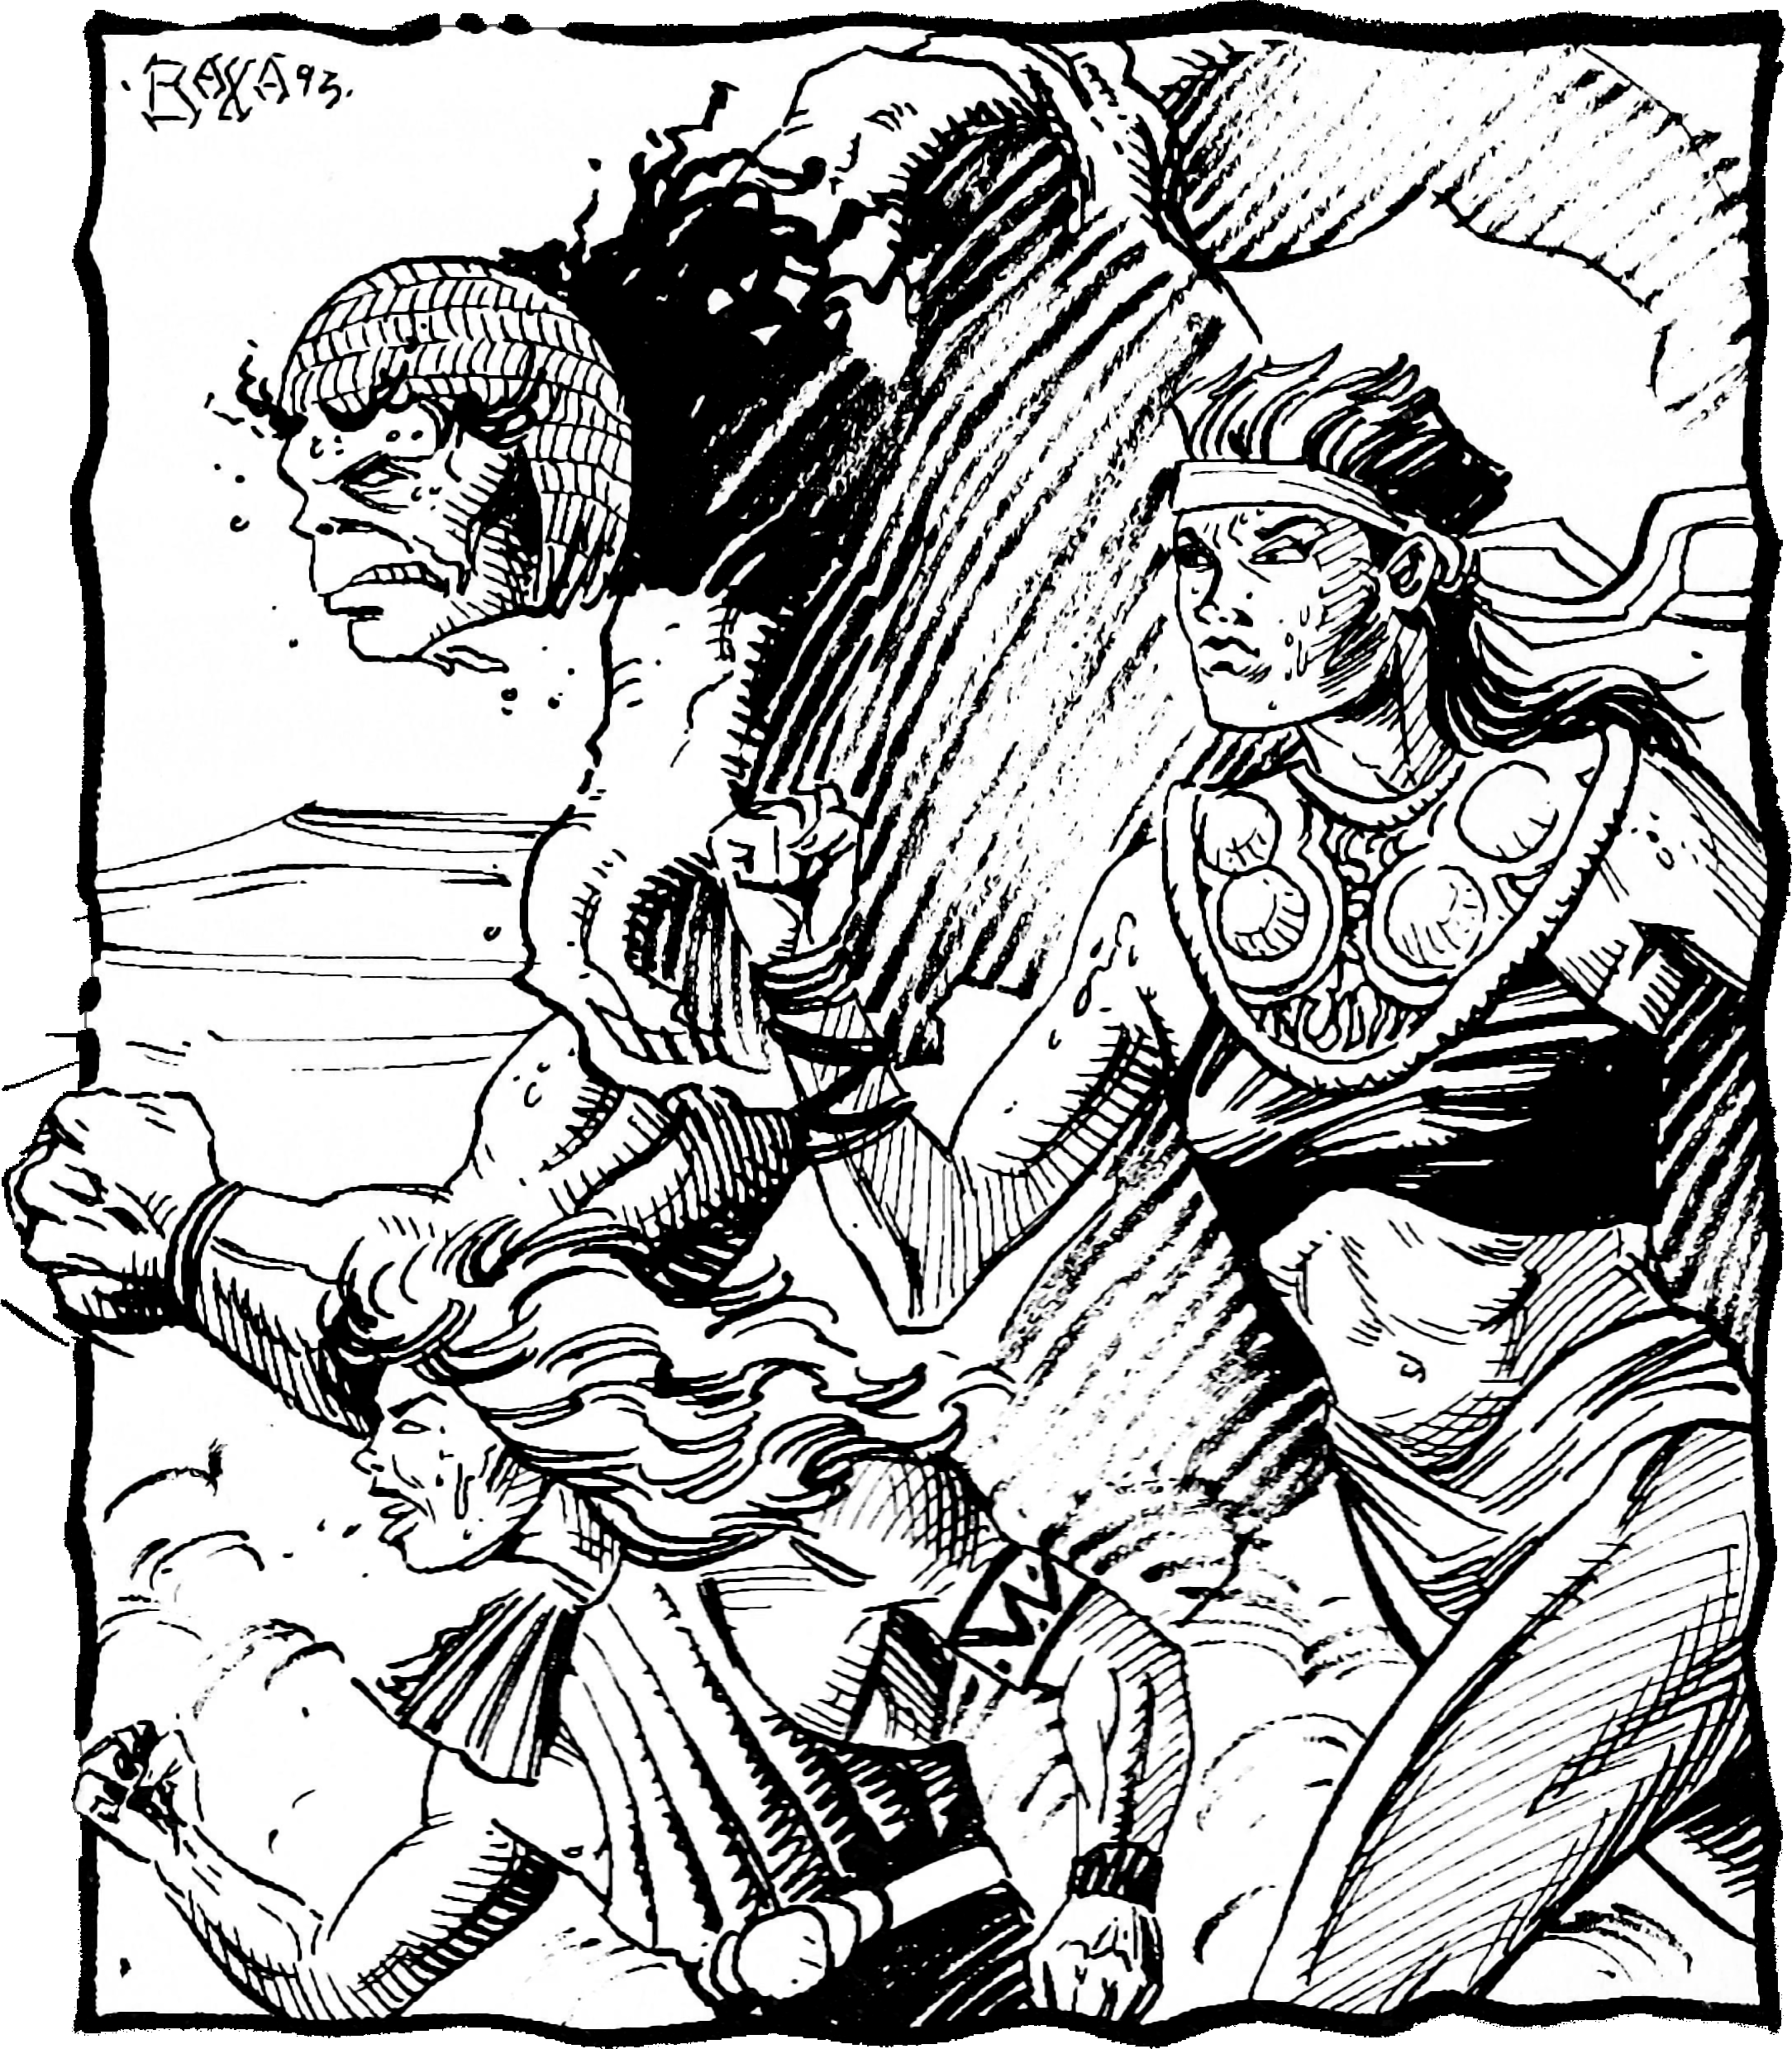
\includegraphics[width=\columnwidth]{images/running-1.png}
\WOTC
\end{figure}
\subsubsection{Run}
You can run as a full-round action. (If you do, you do not also get a 1.5-meter step.) When you run, you can move up to four times your speed in a straight line (or three times your speed if you're in heavy armor). You lose any Dexterity bonus to AC unless you have the \feat{Run} feat.

You can run for a number of rounds equal to your Constitution score, but after that you must make a DC 10 Constitution check to continue running. You must check again each round in which you continue to run, and the DC of this check increases by 1 for each check you have made. When you fail this check, you must stop running. A character who has run to his limit must rest for 1 minute (10 rounds) before running again. During a rest period, a character can move no faster than a normal move action.

You can't run across difficult terrain or if you can't see where you're going.

A run represents a speed of about 18 kilometers per hour for an unencumbered human.

\subsubsection{Move 1.5 meter through Difficult Terrain}
In some situations, your movement may be so hampered that you don't have sufficient speed even to move 1.5 meter (a single square). In such a case, you may spend a full-round action to move 1.5 meter (1 square) in any direction, even diagonally. Even though this looks like a 1.5-meter step, it's not, and thus it provokes attacks of opportunity normally.